% Source: AESP_466_ClassWork/Supplements/Notes/latex/6.6.1/6.6.1.tex

\documentclass[border=4pt]{standalone}
\usepackage{amsmath,amssymb,amsthm}
\usepackage{graphicx}
\usepackage{tikz}
\usepackage{xcolor}
\usetikzlibrary{arrows.meta,calc,positioning,decorations.markings,patterns,shapes.geometric,angles,quotes}

\definecolor{Garnet}{HTML}{73000A}
\definecolor{USC_Rose}{HTML}{CC2E40}
\definecolor{USC_Blue}{HTML}{466A9F}
\definecolor{USC_Slate}{HTML}{1F414D}
\definecolor{USC_Olive}{HTML}{65780B}
\definecolor{USC_Lime}{HTML}{CED318}
\definecolor{USC_Gold}{HTML}{A49137}
\definecolor{USC_Black90}{HTML}{565556}
\definecolor{USC_Black10}{HTML}{ECECEC}

\newcommand{\vect}[1]{\mathbf{#1}}
\newcommand{\mat}[1]{\mathbf{#1}}
\newcommand{\uvec}[1]{\hat{\mathbf{#1}}}
\newcommand{\transpose}{^{\mkern-1.5mu\mathsf{T}}}
\newcommand{\inv}{^{-1}}
\newcommand{\deriv}[2]{\frac{d #1}{d #2}}
\newcommand{\pderiv}[2]{\frac{\partial #1}{\partial #2}}

\begin{document}
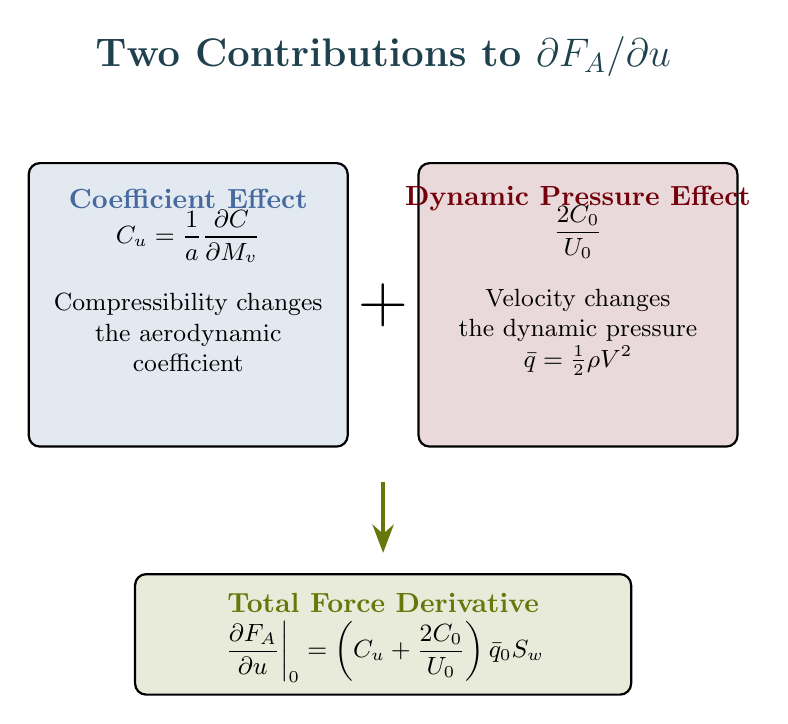
\begin{tikzpicture}[>=Stealth, scale=0.9]
    % Title
    \node[font=\Large\bfseries, USC_Slate] at (5,5.5) {Two Contributions to $\partial F_A/\partial u$};

    % Left box - Coefficient effect
    \draw[thick, fill=USC_Blue!15, rounded corners] (0,0) rectangle (4.5,4);
    \node[font=\bfseries, USC_Blue] at (2.25,3.5) {Coefficient Effect};
    \node[align=center, font=\small] at (2.25,2.2) {$C_u = \dfrac{1}{a}\dfrac{\partial C}{\partial M_v}$\\[10pt]
    Compressibility changes\\the aerodynamic\\coefficient};

    % Right box - Dynamic pressure effect
    \draw[thick, fill=Garnet!15, rounded corners] (5.5,0) rectangle (10,4);
    \node[font=\bfseries, Garnet] at (7.75,3.5) {Dynamic Pressure Effect};
    \node[align=center, font=\small] at (7.75,2.2) {$\dfrac{2C_0}{U_0}$\\[10pt]
    Velocity changes\\the dynamic pressure\\$\bar{q} = \frac{1}{2}\rho V^2$};

    % Plus sign
    \node[font=\Huge] at (5,2) {$+$};

    % Arrow to result
    \draw[->, ultra thick, USC_Olive] (5,-0.5) -- (5,-1.5);

    % Result box
    \draw[thick, fill=USC_Olive!15, rounded corners] (1.5,-3.5) rectangle (8.5,-1.8);
    \node[font=\bfseries, USC_Olive] at (5,-2.2) {Total Force Derivative};
    \node[font=\small] at (5,-2.9) {$\displaystyle\left.\pderiv{F_A}{u}\right|_0 = \left(C_u + \frac{2C_0}{U_0}\right)\bar{q}_0 S_w$};

\end{tikzpicture}
\end{document}
